\documentclass[12pt]{article}
\usepackage{graphicx}

% \addtolength{\oddsidemargin}{-.875in}
% \addtolength{\evensidemargin}{-.875in}
% \addtolength{\textwidth}{1.75in}
\addtolength{\oddsidemargin}{-.4375in}
\addtolength{\evensidemargin}{-.4375in}
\addtolength{\textwidth}{0.875in}

% \addtolength{\topmargin}{-.875in}
% \addtolength{\textheight}{1.75in}
\addtolength{\topmargin}{-.4375in}
\addtolength{\textheight}{0.875in}

\author{Jim Pivarski}
\date{October 3, 2002}
\title{A--Exam Questions}

\def\lep{{\sc Lep}}
\def\aleph{{\sc Aleph}}
\def\lthree{{\sc L3}}
\def\cdf{{\sc Cdf}}
\def\dzero{{\sc D0}}
\def\slac{{\sc Slac}}
\def\sld{{\sc Sld}}
\def\lhc{{\sc Lhc}}
\def\qqbar{q\={q}}
\def\ccbar{c\={c}}
\def\bbbar{b\={b}}
\def\ttbar{t\={t}}
\def\inv{$^{\mbox{\scriptsize -1}}$}

\begin{document}

\setcounter{section}{1}

\section{Richie's Question}

\begin{quote}
a) Review the current experimental constraints on the mass of the
Standard Model Higgs. What experiments are involved, what did they
measure, and how does their measurement constrin the Higgs mass?
You'll find that \lep\ and \sld\ measured a number of quantities that
help constrain the Higgs mass; focus on the quantities that are most
powerful.

b) For what range of Higgs masses is discovery within reach of the
Tevatron or the \lhc? Which processes are these experiments planning to
use in their searches, and why?
\end{quote}

\subsection{Standard Model Higgs Boson}

The literature on Higgs bosons is complicated by discussion of what
must be dozens of different Higgs theories, when all
mutually-compatible combinations are considered together. Not only are
(Minimally) Supersymmetric Higgs particles as seriously considered and
sought after as the Standard Model Higgs, there is room to complicate
the theory with new Higgses put in by hand (a ``Higgs Sector''),
either for the sake of generality or to solve the Strong CP Problem.
This write-up assumes a very useful but hard to apply cut: I will only
consider Standard (Glashow-Weinberg-Salam) Model Higgs Particles.

The Standard Model Higgs particle is a scalar introduced to the
SU(2)$\times$U(1) Lagrangian to address the problem of local gauge
invariance. A na\"{\i}vely-constructed Lagrangian, meant to emulate
real-world electroweak interactions, would include mass terms for the
W and Z bosons. Such terms violate local gauge invariance, making the
model non-renormalizable and therefore meaningless beyond first order.
Instead, a new scalar particle $\phi$ is introduced with a negative
mass-squared, so that the energy-minimizing states are offset from the
$\phi=0$ origin. Perturbation expansions must be made around the
offset point, yielding an effective Lagrangian that has massive gauge
particles. The original Lagrangian has local gauge invariance, making
the theory renormalizable in principle, and the effective Lagrangian
has massive gauge bosons, making the theory agree with experiment.
Fermion masses can also be generated by adding terms that couple them
to the scalar field $\phi$. This $\phi$ is the Higgs boson.
([\ref{cite:hm}] chapters 14--15 and [\ref{cite:ps}] chapters 20--21).

\begin{figure}[t]
  \begin{center}
    \begin{tabular}{c c p{0.5cm} c c}
      \begin{minipage}{2cm}
        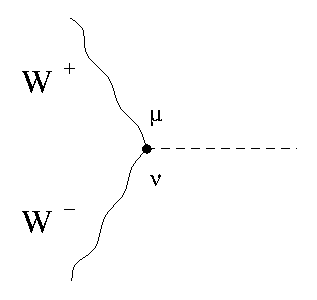
\includegraphics[width=\linewidth]{coupling_higgs-W.eps}
      \end{minipage} &
      \begin{minipage}{4cm}
        $=\ \displaystyle 2i\sqrt{\frac{\lambda}{2}}
             \left(\frac{\mbox{$m_W$}^2}{\mbox{$m_H$}^2}\right)g^{\mu\nu}$
      \end{minipage} & &
      \begin{minipage}{2cm}
        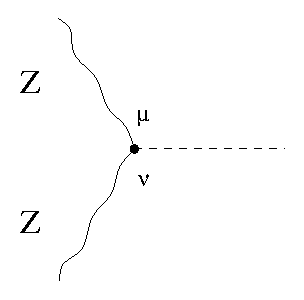
\includegraphics[width=\linewidth]{coupling_higgs-Z.eps}
      \end{minipage} &
      \begin{minipage}{4cm}
        $=\ \displaystyle 2i\sqrt{\frac{\lambda}{2}}
             \left(\frac{\mbox{$m_Z$}^2}{\mbox{$m_H$}^2}\right)g^{\mu\nu}$
      \end{minipage} \\
      & & & & \\
      \begin{minipage}{2cm}
        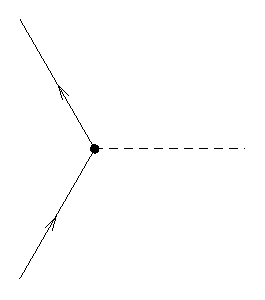
\includegraphics[width=\linewidth]{coupling_higgs-fermion.eps}
      \end{minipage} &
      \begin{minipage}{4cm}
        $=\ \displaystyle -i\sqrt{\frac{\lambda}{2}}
             \left(\frac{\mbox{$m_f$}^2}{\mbox{$m_H$}^2}\right)$
      \end{minipage} & &
      \begin{minipage}{2cm}
        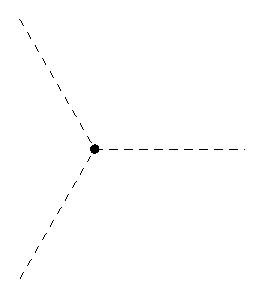
\includegraphics[width=\linewidth]{coupling_higgs-higgs.eps}
      \end{minipage} &
      \begin{minipage}{4cm}
        $=\ \displaystyle -3i\sqrt{\frac{\lambda}{2}}$
      \end{minipage} \\
    \end{tabular}
  \end{center}

  \caption{Feynman-rule couplings for the Higgs boson, predicted by
  the Glashow-Weinberg-Salam model.}

  \label{fig:couplings}
\end{figure}
      
Since this Higgs boson is a new particle (to me), it would help to
list the Feynman rules that connect it to existing particles.
Conveniently, these rules were calculated by Peskin and Schroder
[\ref{cite:ps}] on page 716. They are reproduced in Figure
\ref{fig:couplings}. The Higgs boson is a $\phi^4$ particle, so it
also has the four-point $-12i\lambda$ vertex. (The factor of 12
matches the Higgs definition of $\lambda$ p.~690 with the $\phi^4$
definition of $\lambda$ p.~77.) ((Just from the topology of possible
vertices, the Higgs boson looks like a scalar, massive, colorless
gluon that couples to everything with mass. The analogy probably
doesn't go very deep.))

\subsubsection{Higgs Production}

\begin{figure}[p]
  \begin{center}
    \begin{tabular}[t]{c p{0.5cm} c}
      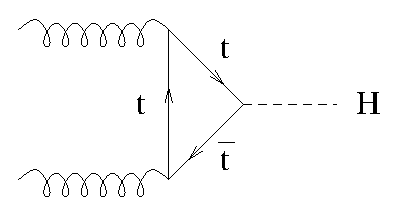
\includegraphics[scale=0.5]{production_gluon_fusion.eps} & &
      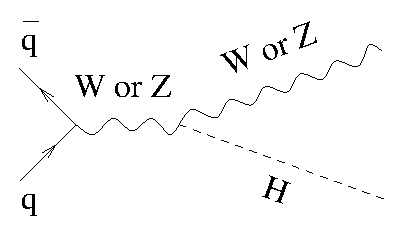
\includegraphics[scale=0.5]{production_higgsstrahlung.eps} \\
      {\bf Gluon Fusion} (gg $\to$ h$_{\mbox{\scriptsize SM}}$) & &
      {\bf Higgsstrahlung} (\qqbar\ $\to$ h$_{\mbox{\scriptsize SM}}$\{W,Z\}) \\
      & \vspace{0.5cm} & \\
      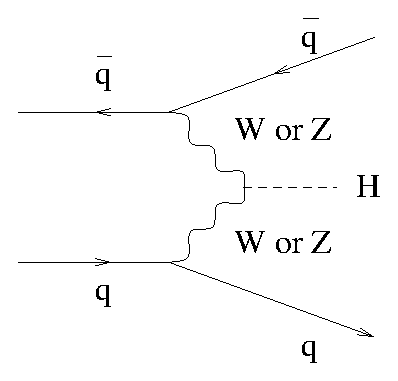
\includegraphics[scale=0.5]{production_vector_boson_fusion.eps} & &
      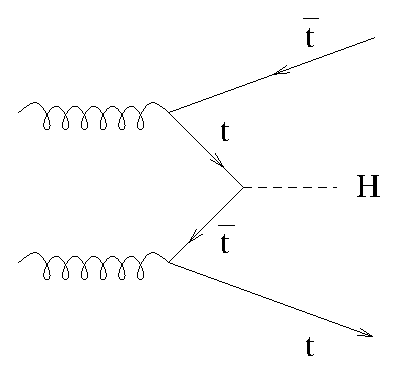
\includegraphics[scale=0.5]{production_tt_fusion.eps} \\
      {\bf Vector Boson Fusion} (\qqbar\ $\to$ h$_{\mbox{\scriptsize SM}}$\qqbar) & &
      {\bf \ttbar\ Fusion} (gg $\to$ h$_{\mbox{\scriptsize SM}}$\ttbar) \\
    \end{tabular}
  \end{center}

  \caption{Principle Higgs production mechanisms for hadron
  colliders.}

  \label{fig:production}
\end{figure}

\begin{figure}[p]
  \begin{center}
    \includegraphics[width=0.8\linewidth]{higgs_production.eps}
  \end{center}

  \caption{Cross-sections for the principle Higgs production
  mechanisms in picobarns, depending on the mass of the Higgs. The
  largest cross-sections correspond to Gluon Fusion (gg $\to$
  h$_{\mbox{\scriptsize SM}}$), Higgsstrahlung (\qqbar\ $\to$
  h$_{\mbox{\scriptsize SM}}$\{W,Z\}) and Vector Boson Fusion (\qqbar\
  $\to$ h$_{\mbox{\scriptsize SM}}$\qqbar).}

  \label{fig:production_xs}
\end{figure}

There are four primary (named) mechanisms for producing Higgs
particles in hadron colliders [\ref{cite:spiwoks}]. These are shown in
Figure \ref{fig:production} and listed here in approximate order of
dominance:
\begin{enumerate}

  \item {\bf Gluon Fusion} produces a single Higgs particle without
  any related (taggable) particles or jets. It is enhanced by the
  coupling of the Higgs to a top quark and suppressed by the three top
  propagators. In the end it wins, with cross-sections ranging from 2
  pb for low $m_H$ to 0.2 pb for high $m_H$.

  \item {\bf Higgsstrahlung} creates a Higgs particle to put a
  virtual W or Z particle on shell. W boson Higgsstrahlung is stronger
  than Z Higgsstrahlung, which is counter-intuitive for several
  reasons. I found phase space differences to be negligible at 2 TeV,
  and the Z boson should have a stronger coupling to the Higgs than
  the W by a factor of 1.3. Even the combinatorics of quarks in a
  proton colliding with an antiproton favor the production of a Z: 5
  wyas to make a Z versus 3 ways to make a W. Nevertheless, W
  Higgsstrahlung is about a factor of two stronger than Z
  Higgsstrahlung, with 0.6 pb (for low $m_H$) to 0.02 pb (for high
  $m_H$).

  \item {\bf Vector Boson Fusion} creates a Higgs particle along with
  two jet-forming quarks through a pair of W's or Z's. The jets help
  to distinguish modes formed via this production mechanism from QCD
  and electroweak backgrounds. The cross-section falls of less
  quickly, from 0.2 pb (at low $m_H$) to 0.3 pb (at high $m_H$).

  \item {\bf \ttbar\ Fusion} creates a Higgs particle with two
  top-quark jets. This process is an order of magnitude less plentiful
  than the others, from 0.01 pb at low $m_H$ to 0.0006 pb at high
  $m_H$. It has as many top-quark vertices as gluon fusion, but it
  needs to make three heavy particles. Naturally, as the Higgs mass
  increases, the probability of this drops. This is the only process
  discussed in the literature which is not (to my knowledge) an option
  considered at the Tevatron or \lhc.

\end{enumerate}

My quotes of production cross-section were read off a plot (Figure
\ref{fig:production_xs}) from the Tevatron contingent of the 2001
Higgs Working Group [\ref{cite:wg_tevatron}]. The center-of-mass
energy is assumed to be 2 TeV.

\subsubsection{Higgs Decay}

\begin{figure}
  \begin{center}
    \includegraphics[width=0.8\linewidth]{higgs_branching_ratios.eps}
  \end{center}

  \caption{Branching ratios for the Higgs boson, depending on its
  mass. The Higgs is unlikely to have a mass above 200 GeV.}

  \label{fig:branching_ratios}
\end{figure}

To know what kinds of signatures to look for, one must also know the
primary decays of the Higgs boson. The branching fractions for these
decays are shown in Figure \ref{fig:branching_ratios} (from
[\ref{cite:hinchliffe}]). The ones of interest (biggest ones) are:
\begin{enumerate}

  \item {\bf b-\={b}} in a low-Higgs mass range ($m_H < \mbox{150
  GeV}$) is by far dominant, about 90\%.

  \item {\bf $\tau$ pairs}, also in the low-mass range, make up most
  of the remaining 10\%. These two contributions remain approximately
  a factor of ten apart through the whole energy range. This is
  satisfactorily close to their coupling ratio of six.

  \item {\bf W pairs} dominate the high-Higgs mass region ($m_H >
  \mbox{150 GeV}$, at one point peaking to 100\% (at the $2m_W$
  threshold). (Below this point, one of the two W bosons is virtual,
  but the branching fraction is still non-negligible.

  \item {\bf Z pairs} come in second for the high-mass Higgs. Above
  the $2m_Z$ threshold, this mode makes up 20--30\% of the decays.

\end{enumerate}

\subsection{Measurements that Constrain the Higgs Mass}

\begin{figure}
  \begin{center}
    \begin{tabular}{c p{0.5cm} c}
      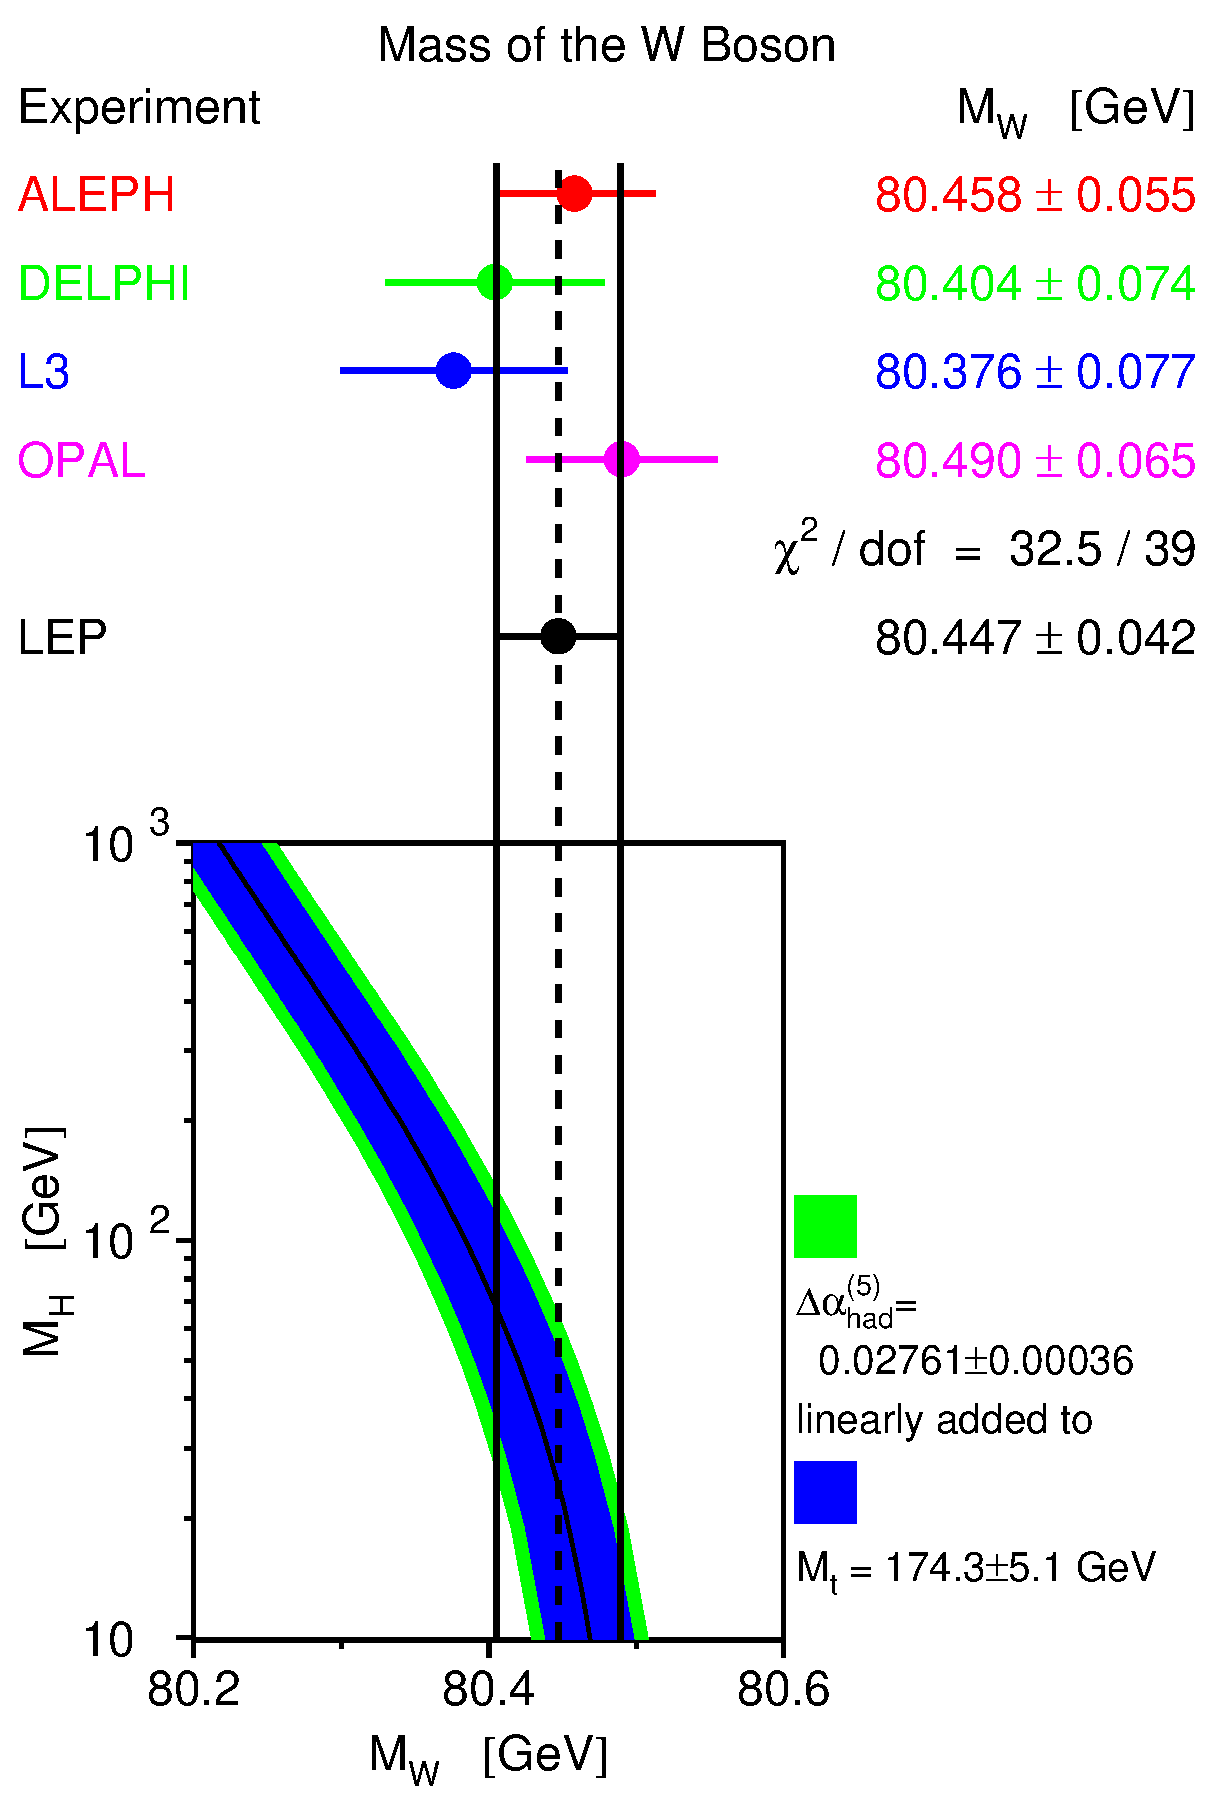
\includegraphics[height=8cm]{s02_mw.eps} & &
      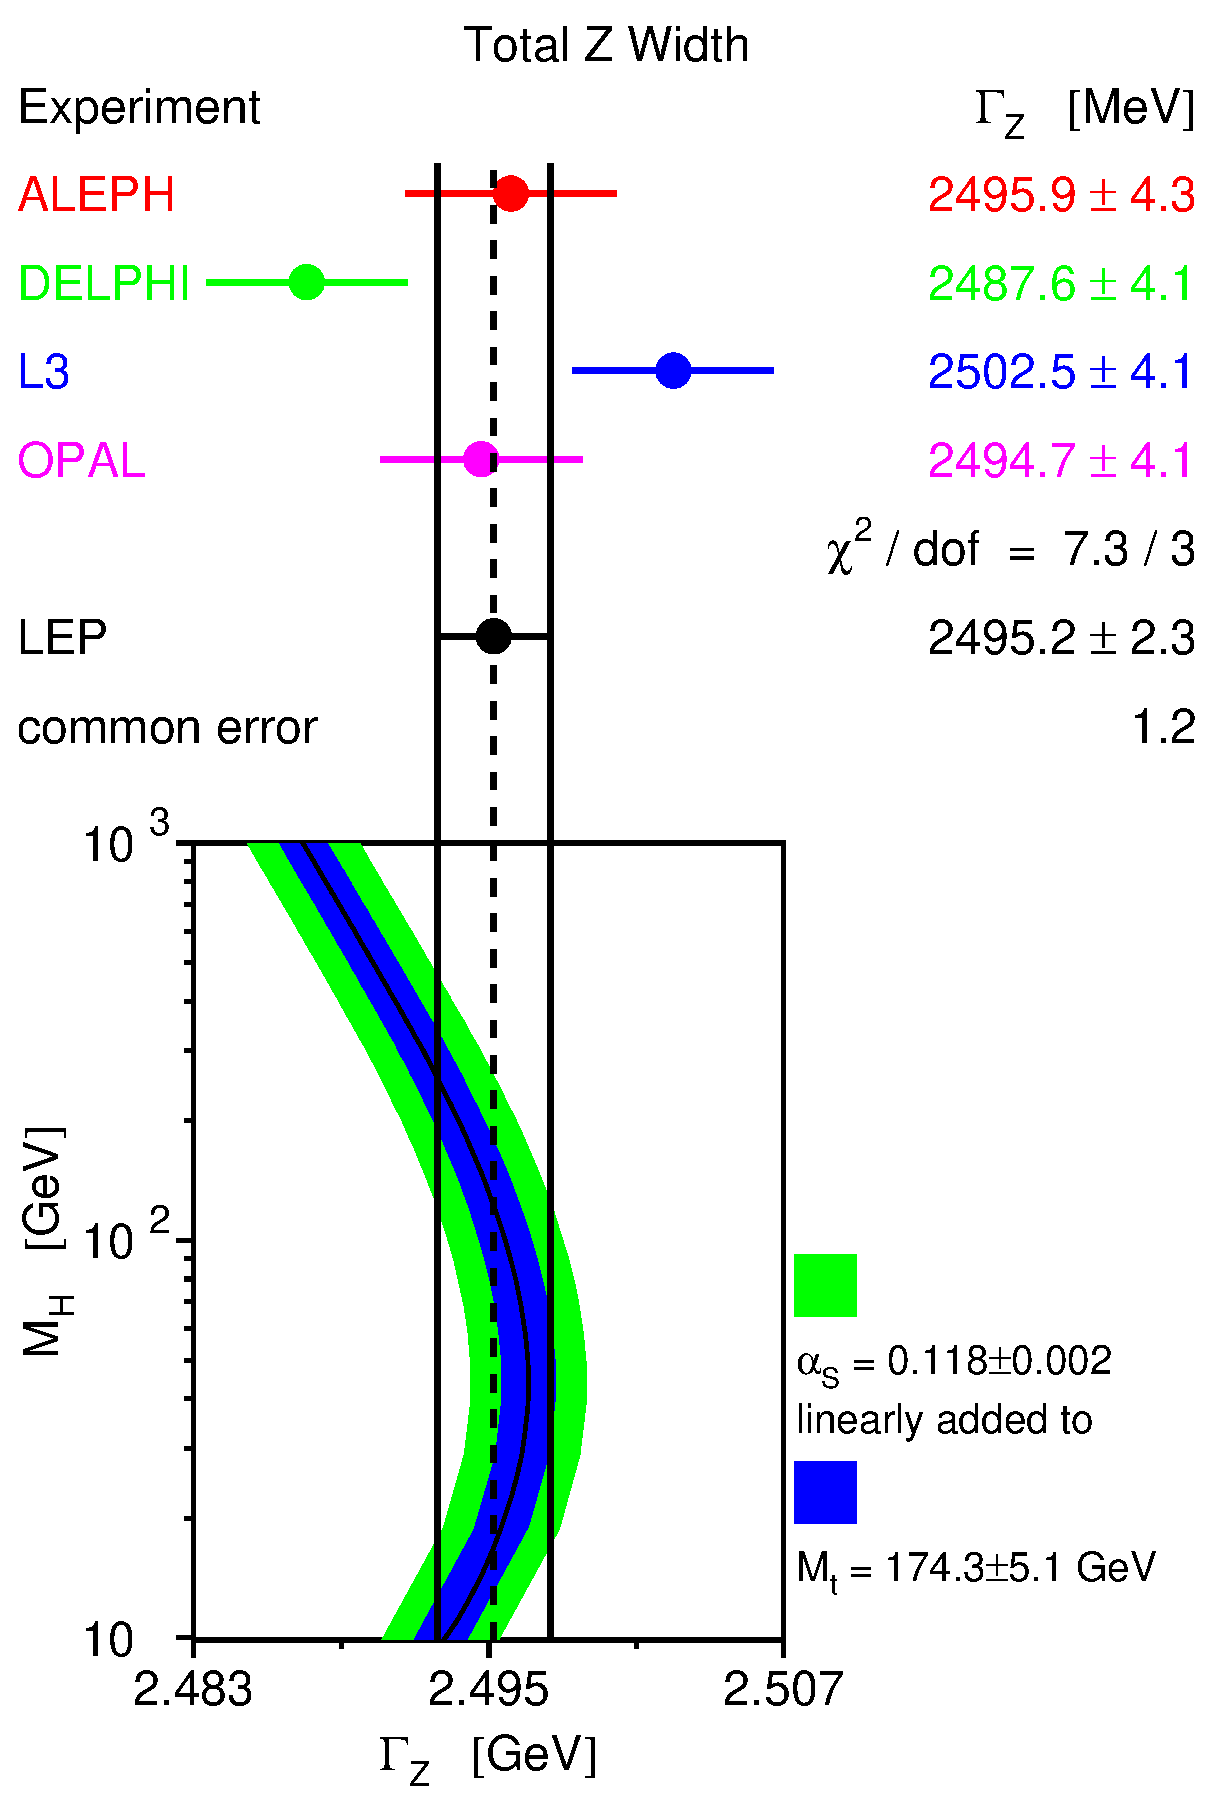
\includegraphics[height=8cm]{lep1_gz.eps} \\
      {\bf Mass of the W Boson (\lep)} & & {\bf Width of the Z Boson (\lep)} \\
      & \vspace{0.5cm} & \\
      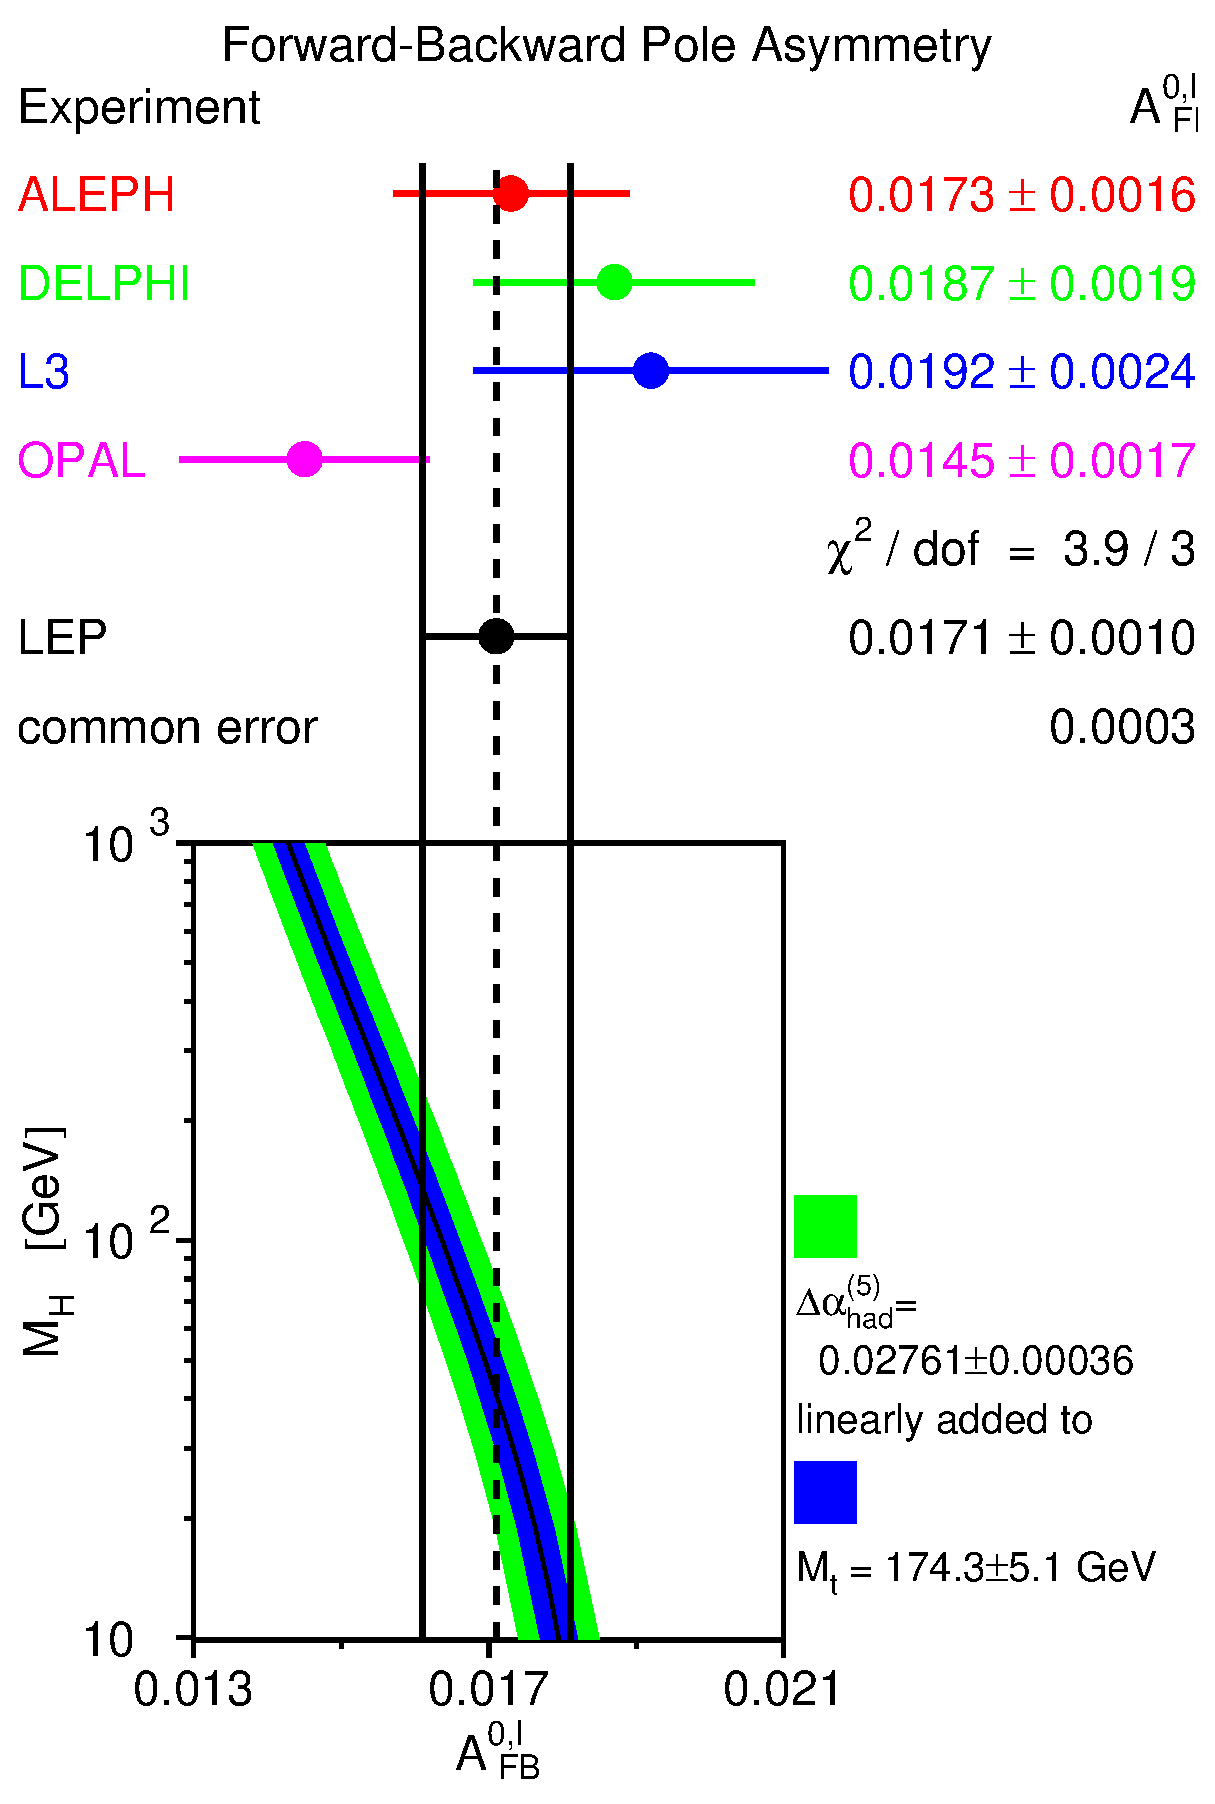
\includegraphics[height=8cm]{lep1_al.eps} & &
      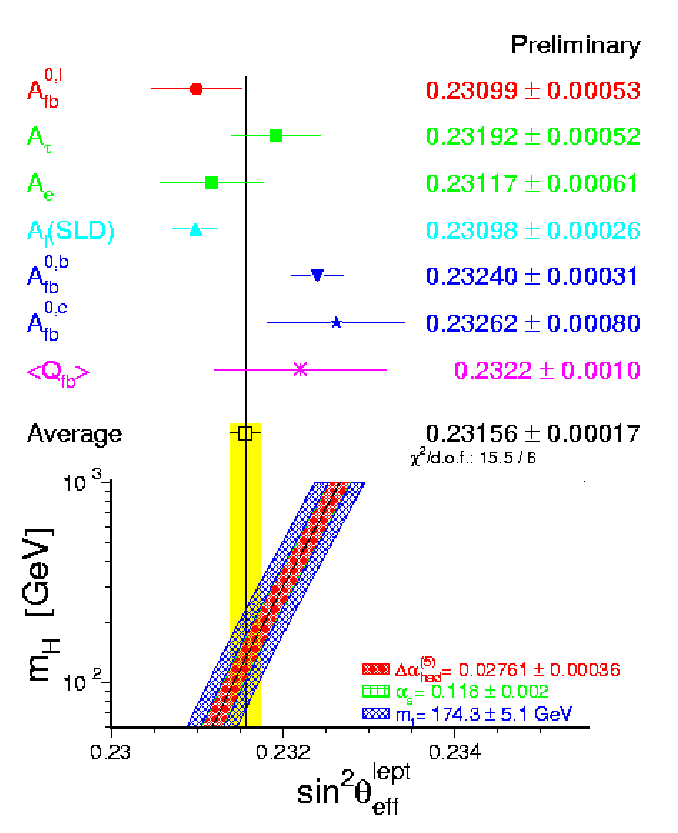
\includegraphics[height=8cm]{sld_al.eps} \\
      {\bf Z-Parity Asymmetry (\lep)} & & {\bf Weak Mixing Angle (\sld)} \\
    \end{tabular}
  \end{center}

  \caption{Three quantities which constrain the Higgs mass, assuming
  the top mass to be 174.3 $\pm$ 5.1 GeV. Z-Parity Asymmetry and the
  Weak Mixing Angle are equivalent--- the fourth figure shows the
  measurement made at \sld.}

\end{figure}

The earliest references that I came across put upper constraints on
the Higgs mass by considering what extremes would cause the
perturbative expansion to break down. More recently, the constraints
have come from precision values of electroweak parameters in analogy
to the way that the top mass was constrained before it was discovered.
When I found \lep's Electro-Weak Working Group page
[\ref{cite:lepewwg}], I scanned the column of plots to find three that
looked the most restrictive on the Higgs boson mass. They are: W mass,
Z width and Z-parity asymmetry. Subsequent remarks discovered in the
literature (for example, in [\ref{cite:sldwewg}]) agree with the first
and third as being interesting, I will focus on them.

\subsubsection{W Boson Mass}

\begin{figure}
  \begin{center}
    \begin{tabular}{p{0.55\linewidth} c p{0.35\linewidth}}
      \begin{minipage}{\linewidth}
        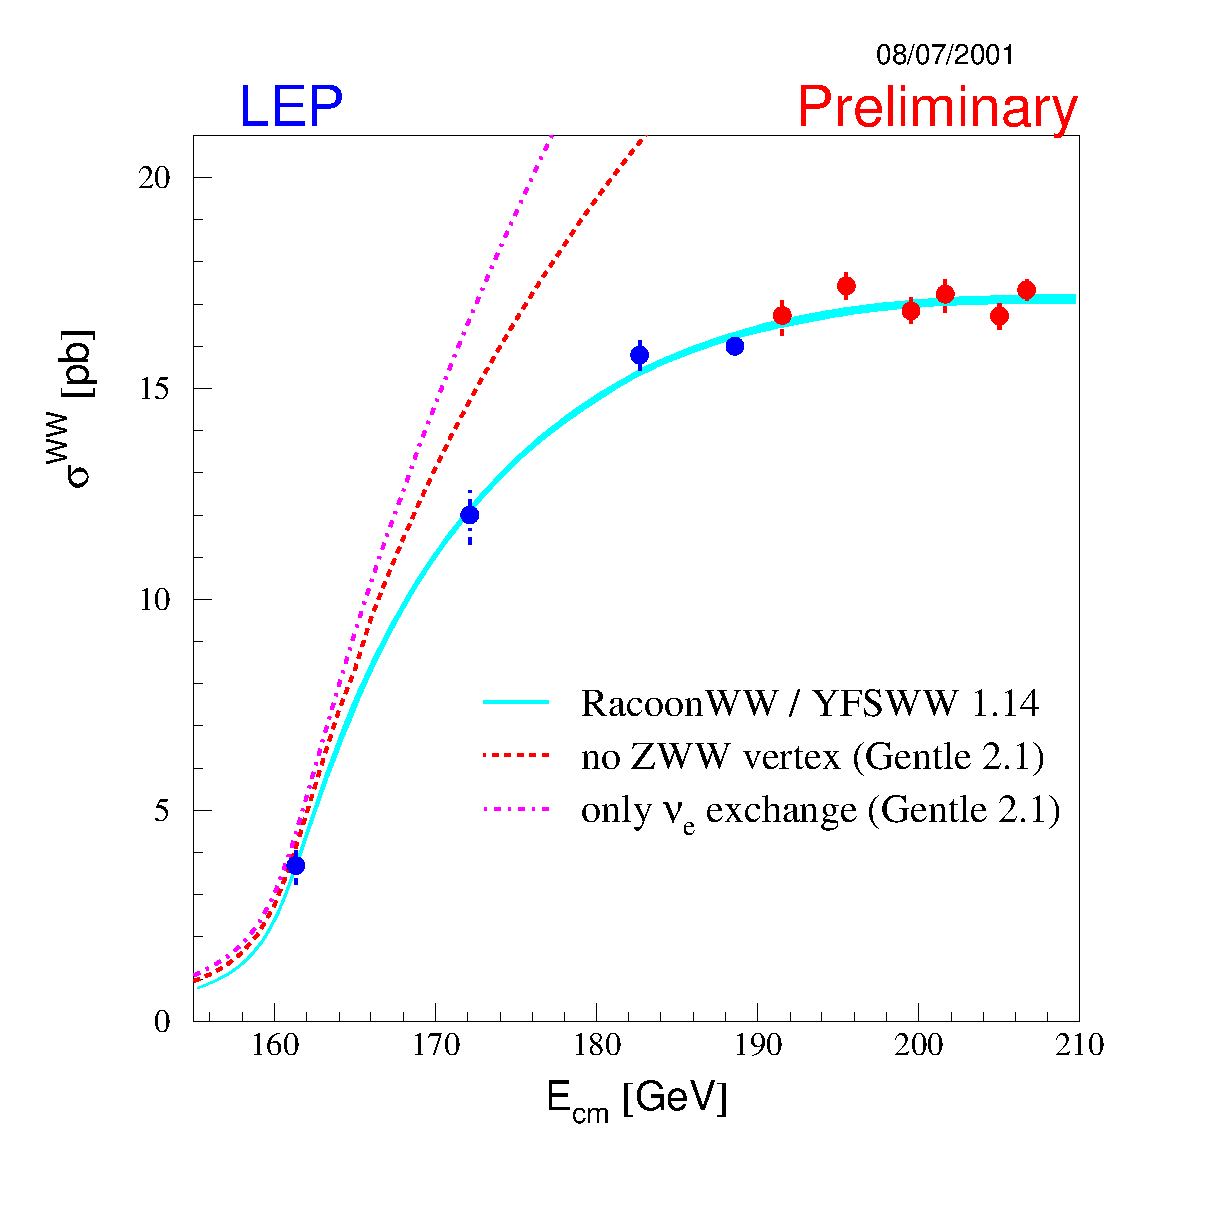
\includegraphics[width=\linewidth]{s01_sww_no_tgc.eps}
      \end{minipage} & &
      \begin{minipage}{\linewidth}

	\caption{The process e$^+$e$^-$ $\to$ W$^+$W$^-$ at threshold,
	a sensitive way to determine the mass of the W boson. The
	upper dotted line corresponds to a simulation using only
	neutrino exchange, the lower dotted line is a simulation using
	neutrino exchange and photon $s$-channel. The full line
	corresponds to two (agreeing) simulations using all three
	diagrams. (All simulations have been corrected for initial
	state radiation.)}

      \end{minipage} \\
    \end{tabular}
  \end{center}

  \label{fig:w_mass}
\end{figure}

Recent (post-1995) data on the mass of the W boson comes from
threshold measurements made at \lep\ and high-energy (high-statistics)
measurements made at \dzero. The \lep\ measurement is more intuitive, so
I will only discuss this one ([\ref{cite:lep_ww}] and
[\ref{cite:lep_ww_anne}]).

The idea behind the threshold measurements is simple: near the
center-of-mass energy of $2m_W$, the e$^+$e$^-$ $\to$ W$^+$W$^-$
cross-section ``switches on'' suddenly. The goal, then, is to map out
this curve--- fits will be very sensitive to the W mass. Between 1996
and 2000, \lep\ scanned over ten sample points, yielding the plot in
Figure \ref{fig:w_mass}.

Three diagrams contribute to e$^+$e$^-$ $\to$ W$^+$W$^-$:
\begin{center}
  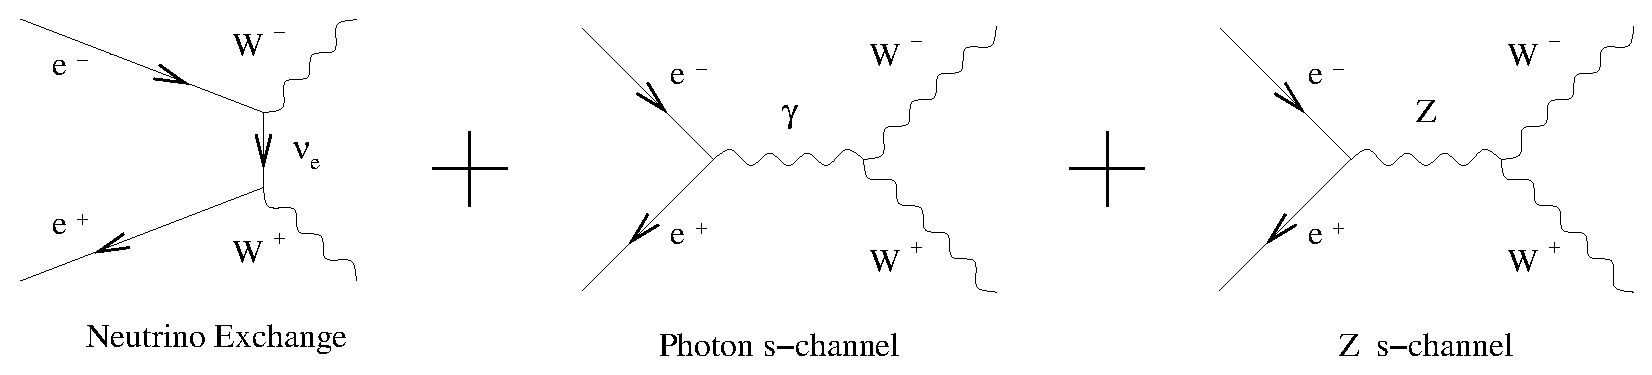
\includegraphics[width=0.8\linewidth]{w_mass_diagrams.eps}
\end{center}
The Figure shows the effect of each diagram on the simulation by
including them one at a time.

The signature for recognizing a W pair event is a final state
consisting of four fermions. Sometimes those fermions are quarks and
therefore jets, so the technique must be divided up into cases:
\begin{enumerate}

  \item $\ell \nu \ell \nu$ (11\%): look for two acoplanar leptons
  with missing energy.

  \item $q\bar{q} \ell \nu$ (44\%): look for two back-to-back jets and
  an isolated lepton or low-multiplicity jet (for $\ell=\tau$) with
  missing energy.

  \item $q\bar{q} q\bar{q}$ (46\%): require no missing energy and
  train a neural net to find the right shape of event. Surprisingly
  (to me), this mode had the highest efficiency and signal-to-noise
  ratio.

\end{enumerate}

The number of observed events were compared to expected events and
combined into a maximum-likelihood fit for $\sigma_{\mbox{\scriptsize
W pair}}$. The cross-sections were plotted as a function of energy (in
Figure \ref{fig:w_mass}) and compared to two simulations: RacoonWW and
YFSWW. In a very similar way to the $\Upsilon$ resonance scans,
initial state radiation spreads the cross-section to higher energies,
so this is incorporated into the fitter.

\subsubsection{Z Width}

\begin{figure}
  \begin{center}
    \begin{tabular}{p{0.55\linewidth} c p{0.35\linewidth}}
      \begin{minipage}{\linewidth}
        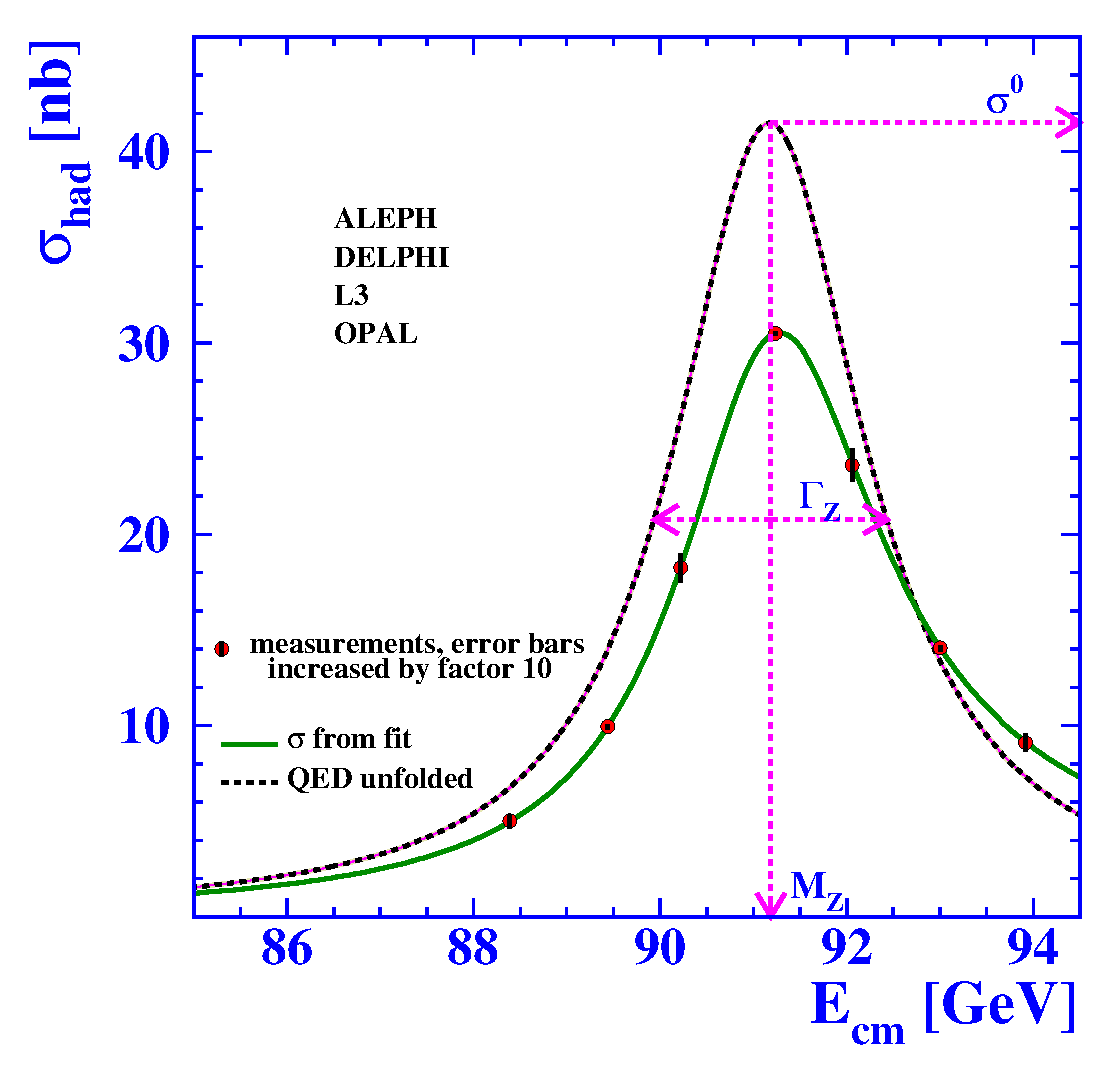
\includegraphics[width=\linewidth]{z_width.eps}
      \end{minipage} & &
      \begin{minipage}{\linewidth}

  	\caption{Resonance scan of the Z boson to determine its width.
  	The solid line is the observed curve (measurement error bars
  	multiplied by 10), the dotted line is a simulation without
  	initial state radiation.}

      \end{minipage} \\
    \end{tabular}
  \end{center}

  \label{fig:z_width}
\end{figure}

Even more similar to the $\Upsilon$ scans is the determination of the
Z boson decay width [\ref{cite:z_width}]. The cross-section of
e$^+$e$^-$ $\to$ q\={q} is measured over a set of energies
near the mass of the Z boson. As is seen in Figure \ref{fig:z_width},
the resulting curve is a Breit-Wigner two and a half GeV wide. The
initial state radiation shifts the peak up in energy and reduces the
cross-section due to smearing.

Any two-fermion final state (except $\nu \nu$) could have been used to
measure the peak, but e$^+$e$^-$ would have been a bad choice,
considering the bhabha background. (Only $\sim$120 pb at this high
energy, but the peak is 30 pb.) The chosen final state was a pair of
quark-jets (70\% of the branching ratio), which has only $s$-channel
components: e$^+$e$^-$ $\to$ $\gamma$ $\to$ q\={q}, e$^+$e$^-$
$\to$ Z $\to$ q\={q} and the interference of the two.

Since the objective is to measure the width of the peak, rather than
the area, uncertainties that don't depend on beam energy, such as the
Z branching ratios, do not contribute to the measurement uncertainty.

\subsubsection{Z Parity Asymmetry}

Since the Z boson is a linear combination of a field that couples with
maximal parity violation ($W_\mu$$^3$) and a field that couples with
no parity violation ($B_\mu$) (Halzen and Martin [\ref{cite:hm}]
p.~336), it couples to fermions with an asymmetry which is closely
related to the weak mixing angle. This parity asymmetry was measured
at \lep\ via forward--backward differences and at \sld\ through
left-handed--right-handed differences. The \sld\ measurement is more
transparent to me, so this is the one I will discuss.

On p.~753 of Peskin and Schroder [\ref{cite:ps}], Feynman-diagram
vertices of Z bosons to left-handed fermions are calculated to be
$\displaystyle \frac{ie\gamma^\mu}{\cos\theta_w \sin\theta_w}
\left(\sin^2\theta_w - \frac{1}{2}\right)$ and to right-handed
fermions: $\displaystyle \frac{ie\gamma^\mu}{\cos\theta_w
\sin\theta_w} \left(\sin^2\theta_w\right)$. 

An experimental quantity which can be directly measured is
\begin{equation}
  A^\ell_{\mbox{\scriptsize L--R}} = \frac{\sigma^\ell_{\mbox{\scriptsize L}} -
    \sigma^\ell_{\mbox{\scriptsize R}}}{\sigma^\ell_{\mbox{\scriptsize L}} + \sigma^\ell_{\mbox{\scriptsize R}}}
  = \frac{\left(\sin^2\theta_w - \frac{1}{2}\right)^2 -
    \sin^2\theta_w}{\left(\sin^2\theta_w - \frac{1}{2}\right)^2 +
    \sin^2\theta_w}
  = \frac{2\left(1 - 4\sin^2\theta_w\right)}{1 + \left(1 -
    4\sin^2\theta_w\right)^2}\mbox{.}
\end{equation}
This provides a direct measurement of $\sin^2\theta_w$ with
polarization-independant factors in the uncertainty cancelling.
$\sigma^\ell_{\mbox{\scriptsize L}}$ is the cross-section for a left-handed
electron to scatter off an unpolarized positron, through a Z boson
$s$-channel to produce lepton $\ell$. Another analysis of the same
experiment considers hadronic final states.

To do the measurement, \sld\ required a polarized beam: the electron
beam was polarized near the source by Compton-scattering off a highly
polarized laser. By the time the beam reached the detector, it was
measured to be 75\% longitudinally polarized. The positron beam was
left unpolarized, and was at one point measured to be so, to high
precision.

$A^\ell_{\mbox{\scriptsize L--R}}$ is obtained from the experiment by looking at
the differental cross-section:
\begin{equation}
  \frac{\partial \sigma}{\partial \left(\cos\theta\right)} = f(s)
  \bigg(\left(1 - P_e A^e_{\mbox{\scriptsize L--R}}\right) \left(1 +
  \cos^2\theta\right) + \left(A^e_{\mbox{\scriptsize L--R}} - P_e\right)
  A^\ell_{\mbox{\scriptsize L--R}} 2 \cos\theta \bigg)
\end{equation}
where $P_e$ is the electron polarization. The electron asymmetry
parameter is determined first, and from this $A^\mu_{\mbox{\scriptsize L--R}}$
and $A^\tau_{\mbox{\scriptsize L--R}}$.

I have already mentioned that this measurement could be performed with
leptonic or hadronic final states. A point of concern (or new
physics!) is that the \sld\ asymmetry measurement for leptons
[\ref{cite:sld_leptons}] differs from the hadron
[\ref{cite:sld_hadrons}] measurement by about 3$\sigma$. There is
nothing in the Standard Model to predict such a discrepancy. Most
authors who touched on this point agreed that it is, at this time,
significant, but quickly moved on to Higgs mass predictions. I will do
the same.

\subsubsection{Higgs Mass Constraint}

\begin{figure}
  \begin{center}
    \begin{tabular}{l r}
      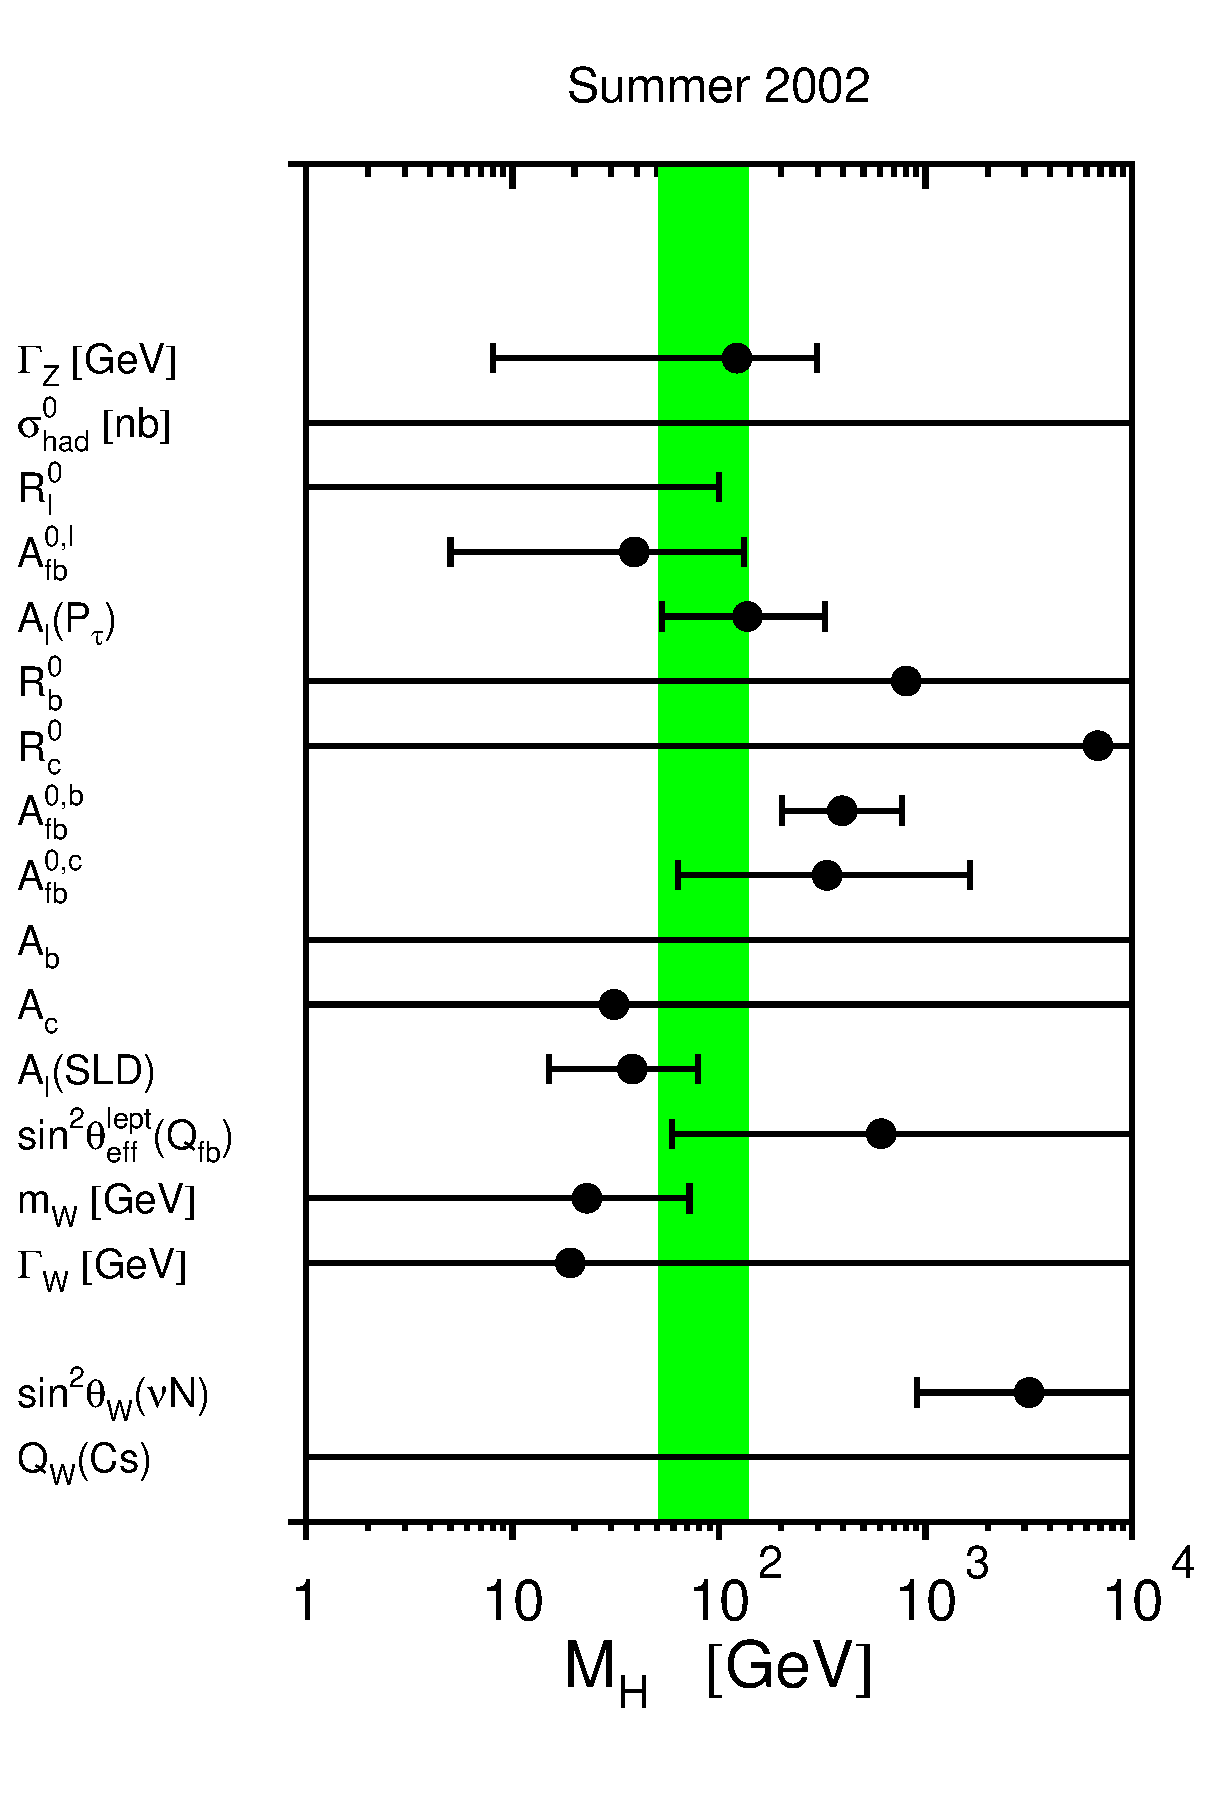
\includegraphics[height=8cm]{s02_show_higgs.eps} &
      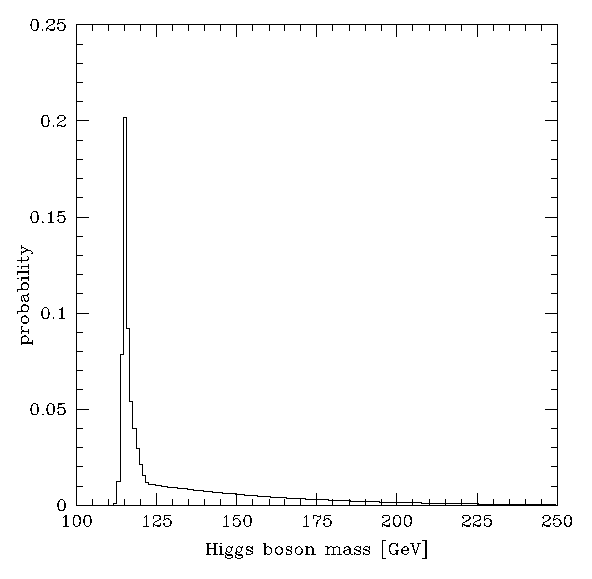
\includegraphics[height=8cm]{mass_pdf.eps} \\
    \end{tabular}
  \end{center}

  \caption{All constraints on the Higgs mass to date place it in a
  region from 50 to 150 GeV. On the right is a probability density
  function for the Higgs mass in 1 GeV bins, given all data (direct
  and indirect) as of October 2000.}

  \label{fig:mass_pdf}
\end{figure}

While they may be the most stringent, these three measurements are not
the only ones restricting the Higgs mass. There are a dozen or two
such measurements, all of which pull the final value of the Higgs mass
to a greater or lesser degree [\ref{cite:lepewwg}]. Taken together,
the set of restrictions on the mass of the Higgs is rather
complicated, so it is nice to see that the state of our knowledge on
the subject has been computed as a probability density function
[\ref{cite:mass_pdf}]. The most recent combined uncertainties, and a
two-year old probability density function are plotted in Figure
\ref{fig:mass_pdf}. Direct searches have ruled out masses up to 110
GeV, and the highest probabilities lie in the region from 110 GeV to
125 GeV. However, about half of the probability lies above 125 GeV.

\subsection{Higgs Discovery Potential of the Tevatron and \lhc}

A Higgs Working Group summary report [\ref{cite:wg}] collected
strategies for Higgs discovery at the Tevatron and \lhc. Here is a
summary of those plans.

\subsubsection{Signatures used by the Tevatron}

At the time of the Working Group (2001), \cdf\ and \dzero\ {\sc Run II}
simulators had not been completed, but quantitative results could be
obtained by extending {\sc Run I} simulators to the wider acceptance
of the {\sc Run II} detectors [\ref{cite:wg_tevatron}].

One significant improvement over {\sc Run I} was assumed: that the
14--15\% \bbbar\ mass resolution can be reduced to 10\%. It was also
assumed that {\sc Run II} b-tagging efficiency would match that of
{\sc Run I}.

Detection strategies depend on the preferred decay mode of the Higgs
boson, and therefore on its mass. Strategeies can be divided into
low-mass ($m_H < \mbox{135 GeV}$) and high-mass.

\vspace{\parskip}

\begin{tabular}{p{0.3\linewidth} p{0.6\linewidth}}
  \begin{minipage}{\linewidth} \centering 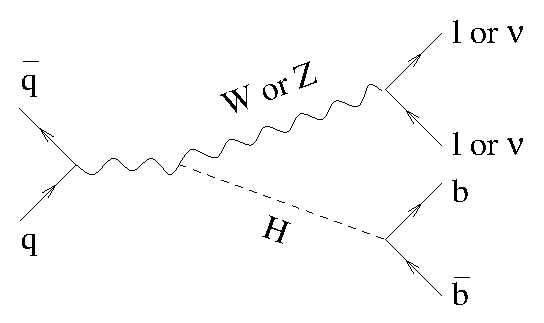
\includegraphics[scale=0.4]{signature_LA.eps} \end{minipage} &

  \begin{minipage}{\linewidth}

    Low-mass Higgs signatures are $\ell \nu \mbox{b\={b}}$, $\nu
    \bar{\nu} \mbox{b\={b}}$ and $\ell^+ \ell^- \mbox{b\={b}}$. They
    come from a Higgsstrahlung production process ($\sim$0.3 pb, see
    Figure \ref{fig:production_xs}), where the associated W or Z
    decays leptonically (30\% of W's, 10\% of Z's). The Higgs boson
    decays into \bbbar, as it is below W pair threshold. Allowing for
    hadronic decays of the vector boson would open a flood of QCD
    backgrounds.

  \end{minipage}
\end{tabular}

\vspace{\parskip}

\begin{tabular}{p{0.3\linewidth} p{0.6\linewidth}}
  \begin{minipage}{\linewidth} \centering 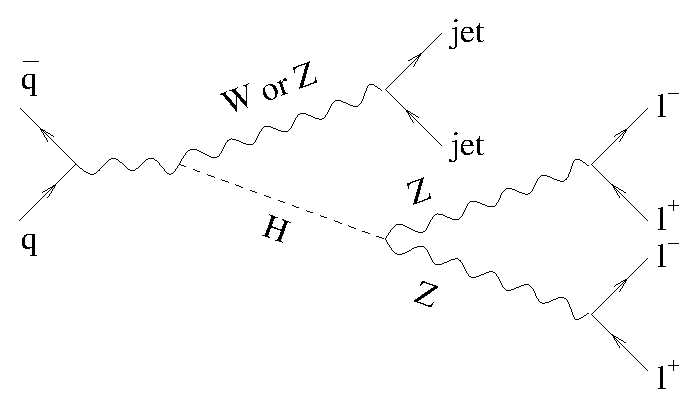
\includegraphics[scale=0.4]{signature_HB.eps} \\
  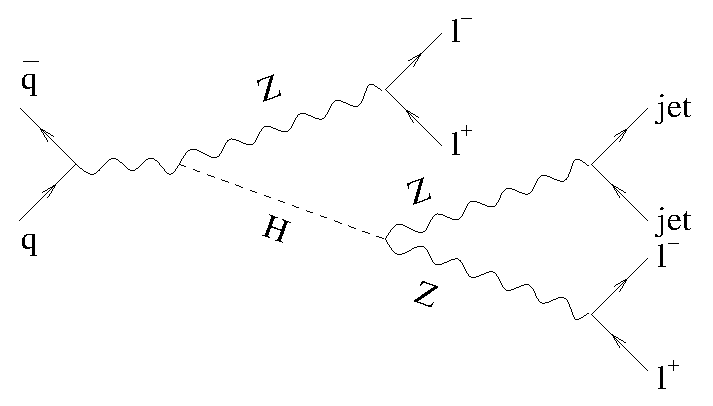
\includegraphics[scale=0.4]{signature_HB2.eps} \end{minipage} &

  \begin{minipage}{\linewidth}

    One high-mass signature is $\ell^\pm \ell^\pm \mbox{ jet jet}$. It
    comes from the distinctive feature of Higgsstrahlung to produce
    triple-vector boson states. The Z boson Higgsstrahlung process is
    $\sim$0.1 pb, and two Z bosons are required to decay leptonically,
    introducing a factor of 1\%. This method will need to be
    supplimented. \\

    \vspace{\parskip}
    A critical issue in this technique is to have an accurate
    estimation of the W + jets and Z + jets backgrounds.

  \end{minipage}
\end{tabular}

\vspace{\parskip}

\begin{tabular}{p{0.3\linewidth} p{0.6\linewidth}}
  \begin{minipage}{\linewidth} \centering 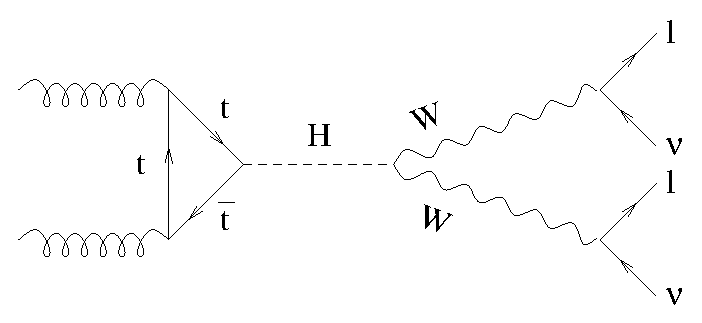
\includegraphics[scale=0.4]{signature_HC.eps} \end{minipage} &

  \begin{minipage}{\linewidth}

    Another high-mass signature is $\ell \bar{\nu} \bar{\ell} \nu$. It
    comes from the much-more-efficient gluon fusion production
    mechanism ($\sim$0.5 pb) but decays as an ordinary W pair, with no
    tag to distinguish it. Therefore, a critical issue with this
    signature is to have an accurate estimation of the electroweak W
    pair background.

  \end{minipage}
\end{tabular}

\vspace{\parskip}

\subsubsection{Signatures used by \lhc}

The \lhc\ document [\ref{cite:wg_lhc}] was much more quantitative, as
they already had a working event simulator. I have no reason to
believe that the \lhc\ Collaboration won't use the same signature
processes that were proposed by the Tevatron committee, but they
proposed a set of measurements using the vector boson fusion
production mechanism, perhaps in addition. This mechanism has
$\sim$0.1 pb for all Higgs masses.

The advantage of using this mechanism is the distinctive pattern of
jets produced by the associated \qqbar\ (see Figure
\ref{fig:production}). Two jets are found in the forward region of the
detector and little jet activity takes place in the central region.

\vspace{6mm}

\begin{tabular}{p{0.3\linewidth} p{0.6\linewidth}}
  \begin{minipage}{\linewidth} \centering 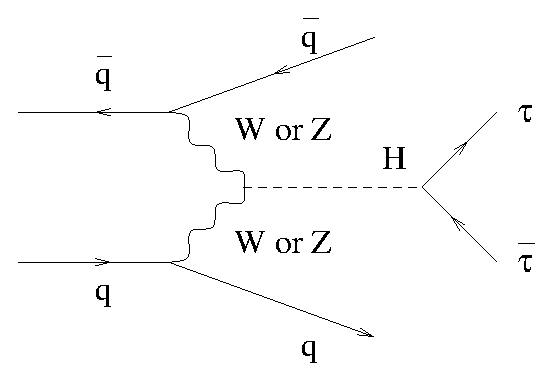
\includegraphics[scale=0.4]{signature_LB_correct.eps} \end{minipage} &

  \begin{minipage}{\linewidth}

    For a low-mass Higgs, produce via vector boson fusion and let the
    Higgs decay into tau pairs ($\sim$10\%, see Figure
    \ref{fig:branching_ratios}). The tau pairs are identified by $ee$,
    $\mu\mu$ and $e\mu$ final states (9\% of tau pairs). The major
    background is Z $\to$ $\tau^+\tau^-$ $\to$ $\ell$ + hadron. The
    signal above the background for a full 30 pb\inv\ dataset is shown
    in Figure \ref{fig:tau_backgrounds}. \\

    \vspace{\parskip}
    Alternatively, a hadronic decay can be accepted on one side of the
    tau pair: a signature of $\ell\nu\bar{\nu}\,\mbox{h}\nu$ + two jets.
    This data is unplotted, but discussed in tabular form later on.

  \end{minipage} \\
\end{tabular}

\vspace{6mm}

\begin{tabular}{p{0.3\linewidth} p{0.6\linewidth}}
  \begin{minipage}{\linewidth} \centering 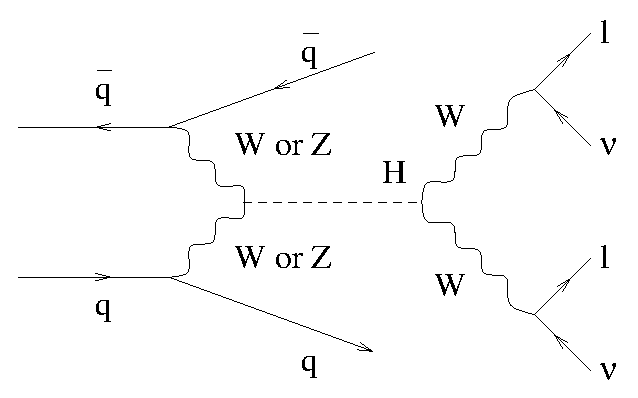
\includegraphics[scale=0.4]{signature_HA_correct.eps} \end{minipage} &

  \begin{minipage}{\linewidth}

    For a high-mass Higgs, produce via vector boson fusion and let the
    Higgs decay into W pairs ($\sim$90\%). There is no choice with W
    pairs: the signature will be $\ell \bar{\nu} \bar{\ell} \nu$ + two
    jets. Before cuts, the cross-section $\sigma_{\mbox{\scriptsize
    production}} \times \mathcal{BR}_{\mbox{\scriptsize W pairs}}$ is
    1.5--3.0 pb and the major backgrounds are 55.0 pb (\ttbar) and
    16.7 pb (QCD W pairs + jets).

  \end{minipage} \\
\end{tabular}

\vspace{6mm}

\begin{figure}
  \begin{center}
    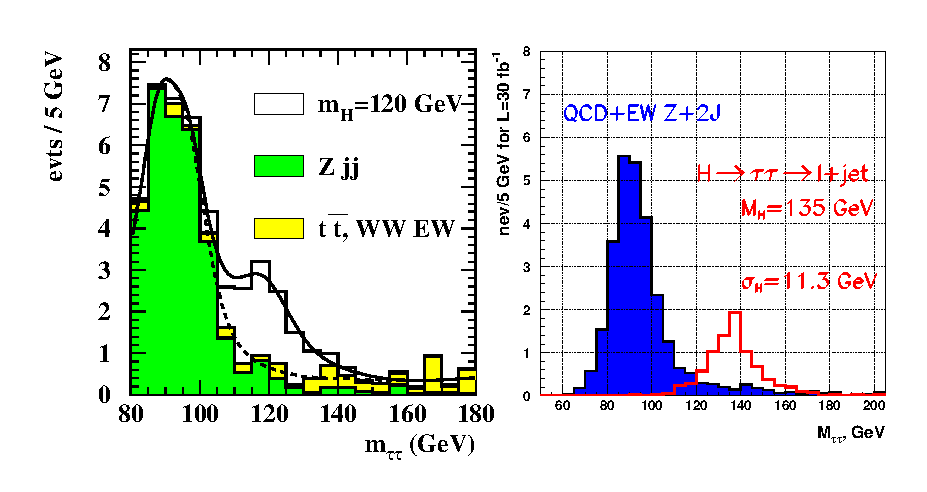
\includegraphics[width=\linewidth]{lhc_higgs_tau_backgrounds.eps}
  \end{center}

  \caption{\lhc\ simulations showing the extraction of a 120 or 135
  GeV Higgs boson using the vector boson fusion Higgs $\to$ $\tau\tau$
  $\to$ $ee$, $\mu\mu$ or $e\mu$ + X with 30 fb\inv\ of data. Tau
  decays to $\ell \nu \nu$ h$\nu$ are not included.}

  \label{fig:tau_backgrounds}
\end{figure}

\begin{figure}
  \begin{center}
    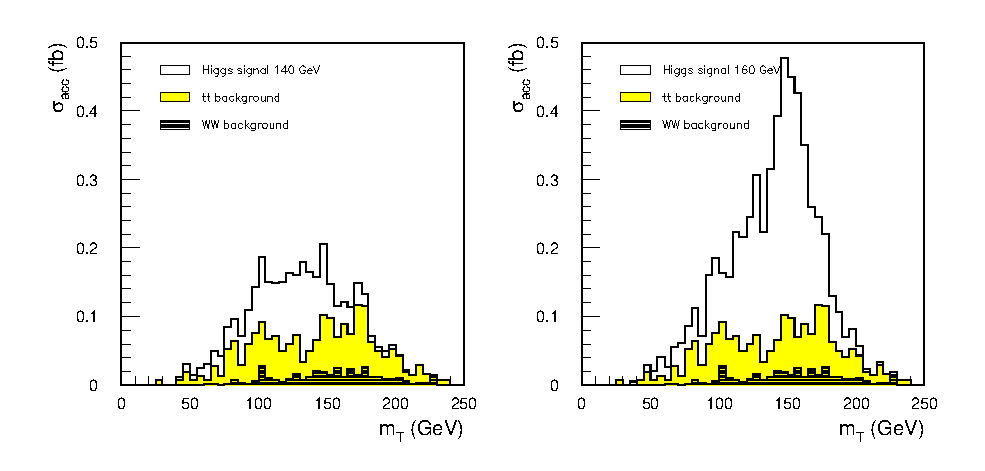
\includegraphics[width=\linewidth]{lhc_higgs_backgrounds.eps}
  \end{center}

  \caption{\lhc\ simulations showing the extraction of a 140 or 160
  GeV Higgs boson using the vector boson fusion Higgs $\to$ W-pair method.
  To determine the event rate, multiply the integrated luminosity to
  the cross-section on the vertical axis (5 or 30 fb\inv).}

  \label{fig:WW_backgrounds}
\end{figure}

Since all of these analyses depend on an unknown parameter--- the
Higgs mass--- the results are not easily summarized, except in tabular
format.

\pagebreak

For a low-mass Higgs, using H $\to$ $\tau^+\tau^-$ $\to$ $\ell \bar{\nu}
\bar{\ell} \nu$,
\begin{center} \includegraphics{table_lhc_low_mass1.eps} \end{center}

For a low-mass Higgs, using H $\to$ $\tau^+\tau^-$ $\to$ $\ell \nu
\bar{\nu}\,\mbox{h}\nu$,
\begin{center} \includegraphics{table_lhc_low_mass2.eps} \end{center}

For a high-mass Higgs, using H $\to$ W$^+$W$^-$,
\begin{center} 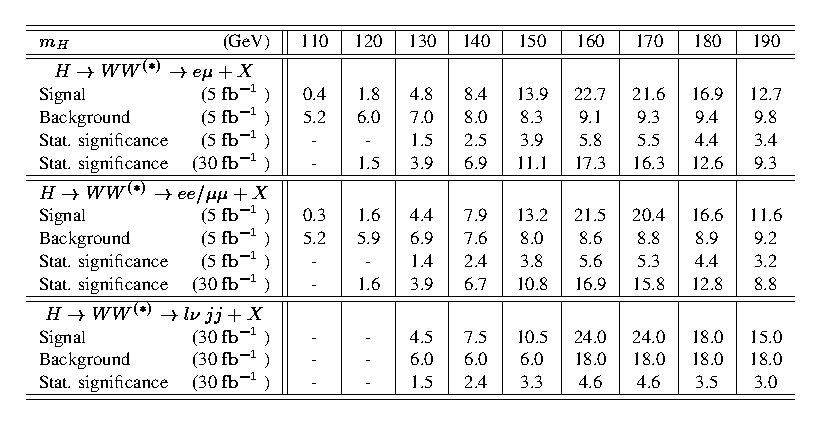
\includegraphics{table_lhc_high_mass.eps} \end{center}

\subsubsection{Tevatron and \lhc\ Discovery Predictions}

So what's the bottom line? The Tevatron can exclude the existance of a
Higgs boson up to 190 GeV at the 95\% confidence level, or discover
one up to 120 GeV at the 5$\sigma$ level [\ref{cite:wg_tevatron}]. The
gluon fusion $\to$ W pair signature is predicted elsewhere to be a
3$\sigma$ discovery level for energies between 148 and 172 GeV
[\ref{cite:wg_supplemental}]. The primary limitation here is \cdf\ and
\dzero's combined integrated luminosity of 15 fb\inv.

The \lhc's prospects look much better [\ref{cite:wg_lhc}]. Using just
the vector boson fusion signatures, they predict a 5$\sigma$ discovery
level for a Higgs mass between 150--185 GeV, using only 5 of the
expected 30 fb\inv\ of data. If all the luminosity is used, a
5$\sigma$ discovery level is predicted for the wider mass range of
130--190 GeV.

The low-Higgs mass signature (tau pairs), requires the full data set
for a clean result, but it is interesting for reasons beyond discovery
potential: it allows for a comparison between generated vector boson
masses (the discovery signature) and generated fermion mass (the tau
coupling strength), which is an entirely different term in the
Lagrangian.

\subsection{References}

\begin{flushleft}
  \begin{enumerate}
  
    \item Halzen and Martin {\it Quarks \& Leptons: An Introductory
    Course in Modern Particle Physics}, John Wiley \& Sons, (1984).
    \label{cite:hm}
  
    \item Peskin and Schroeder {\it An Introduction to Quantum Field
    Theory}, Perseus Books Publishing, L.~L.~C. (1995).
    \label{cite:ps}
  
    \item R. Spiwoks ``Evaluation and Simulation of Event Building
    Techniques for a Detector at the \lhc,'' Dissertation zur Erlangung
    des Grades eines Doktors der Naturwissenschaften der Abteilung
    Physik an der Universit\"at Dortmund, (1995). \\
    {\tt http://rd13doc.cern.ch/RD13/Thesis-Spiwoks/Thesis\_1.html}
    \label{cite:spiwoks}
  
    \item I.~Hinchliffe,
    ``The Higgs Boson: In Review Of Particle Physics (Rpp 1998),''
    Eur.\ Phys.\ J.\ C {\bf 3}, 244 (1998).
    \label{cite:hinchliffe}
  
    \item \lep\ Electroweak Working Group web-site, \\
    {\tt http://lepewwg.web.cern.ch/LEPEWWG/}
    \label{cite:lepewwg}
  
    \item M.~Woods, ``Higgs Mass Predictions via Precision Electroweak Measurements,''
    \slac\ Colloquium (26 Jun 2000). \\
    {\tt http://www-sldnt.slac.stanford.edu/alr/SLAC\_colloq.pdf}
    \label{cite:sldwewg}
  
    \item L.~Malgeri,
    ``W W Cross Sections And W Branching Fractions In L3,''
    Int.\ J.\ Mod.\ Phys.\ A {\bf 16S1A}, 329 (2001).
    \label{cite:lep_ww}
  
    \item A.~Ealet, ``WW Cross Sections and W Branching Ratios,''
    Summer 2000 ICHEP Talk (27 Jul, 2000). \\
    {\tt http://lepewwg.web.cern.ch/LEPEWWG/lepww/4f/doc/osaka\_anne.ps.gz}
    \label{cite:lep_ww_anne}
  
    \item \mbox{[}LEP Collaborations\mbox{]},
    ``Combination procedure for the precise determination of Z boson
    parameters from results of the LEP experiments,''
    [arXiv:hep-ex/0101027].
    \label{cite:z_width}
  
    \item K.~Abe {\it et al.} [SLD Collaboration],
    ``An improved direct measurement of leptonic coupling asymmetries
    with polarized Z bosons,''
    Phys.\ Rev.\ Lett.\  {\bf 86}, 1162 (2001)
    [arXiv:hep-ex/0010015].
    \label{cite:sld_leptons}
  
    \item K.~Abe {\it et al.} [SLD Collaboration],
    ``A high-precision measurement of the left-right Z boson cross-section  asymmetry,''
    Phys.\ Rev.\ Lett.\  {\bf 84}, 5945 (2000)
    [arXiv:hep-ex/0004026].
    \label{cite:sld_hadrons}
  
    \item J.~Erler,
    ``The probability density of the Higgs boson mass,''
    Phys.\ Rev.\ D {\bf 63}, 071301 (2001)
    [arXiv:hep-ph/0010153].
    \label{cite:mass_pdf}
  
    \item D.~Cavalli {\it et al.},
    ``The Higgs working group: Summary report,'' \\
    \mbox{[}arXiv:hep-ph/0203056\mbox{]}, (2002).
    \label{cite:wg}
  
    \item A.~Bocci, J.~Hobbs and W.--M.~Yao, ``B.~Higgs Searches at the
    Tevatron,'' (Published in \ref{cite:wg}).
    \label{cite:wg_tevatron}
  
    \item G.~Azuelos {\it et al.}, ``D.~Search for the Standard Model
    Higgs Boson using Vector Boson Fusion at the \lhc'' (Published in
    \ref{cite:wg}.)
    \label{cite:wg_lhc}
  
    \item T.~Han and R.~J.~Zhang,
    ``Extending the Higgs boson reach at upgraded Tevatron,''
    Phys.\ Rev.\ Lett.\  {\bf 82}, 25 (1999)
    [arXiv:hep-ph/9807424].
    \label{cite:wg_supplemental}
  
  \end{enumerate}
\end{flushleft}

\end{document}



